\section{Background}
\label{background}
\subsection{Failure Repair and Multipath Routing}
Nowadays, network component failures have become routine events rather than exceptions.
Both the industry and the academia have paid attention to improving the network resilience,
and proposed various schemes from physical level methods such as optical routing protection,
to IP level approaches such as IP Fast Rerouting (IPFRR)\cite{IPFRR} that
has been standardized by the IETF. The basic idea of IPFRR is that,
when a node detects the failure of a link directly connected to itself,
it can immediate switch to backup paths that are specifically computed for this failure.
Based on this framework, the following two categories of rerouting mechanisms have been proposed.

The first category works in a local manner. Besides the primary next hop for forwarding
packets to a given destination, a node computes and stores
some alternative next hop, and chooses the alternate when the primary one will fail to work.
Since there is no global cooperation, the alternates have to be selected carefully,
so that no routing loop will be introduced.
The IETF standard \cite{LFA} defines specific rules for selecting such Loop Free Alternates (LFAs),
and we will introduce more details about them in the following subsections.
However, naively computing LFAs with these rules require multiple rounds of
shortest path tree (SPT) computation, and the cost increases proportionally with the
degree of a node, i.e., one SPT for each neighbor.
TBFH \cite{TBFH} and DMPA \cite{dmpa} achieve faster computation at the cost of tightening
the selection rules and less alternates being found.
FIR \cite{20071710572557} improves the protecting capability against a single link failure
by computing different alternates for packets from different incoming ports,
at the cost of an  increased computation overhead, and a restricted scenario,
i.e., only for protecting a link.

The second category computes a multi-hop repair path and requires explicit cooperation or
signaling between routers to ensure packets are indeed routed along this path.
Multi-topology routing\cite{apostolopoulos2006using, gjessing2006implementation} computes routes
on different backup network topologies tailored for specific failures, i.e.,
by removing the corresponding links or by increasing their associated weights.
Routers control which topology they activate by changing additional bits in the packet headers.
FCP \cite {20075110977789} carries link failure information in the IP Packet header
to allow routers to diagnose problems and select alternate paths.
%However, this scheme also requires considerable overhead to find the new working path
%when receiving a packet carrying root-cause failure messages.
Not-via \cite{not-via}\cite{20102012943182}\cite{Menth20101300} uses special not-via addresses
in establishing multi-hop protecting paths.
TOD \cite{Yang2018Fast} proposes tunneling on demand (TOD) to handle one or dual link failures,
but needs it additional signaling protocol to establish tunnels.

Besides failure repair, alternate next hops also find applications in multipath
routing,
where multiple next hops can increase the bandwidth utilization, achieve load balancing, or
improve routing resilience and reliability, if loop free are guaranteed\cite{andersen2002resilient}.
Equal-Cost Multipath Routing (ECMP) \cite{moy1998rfc} allows packets to be forwarded
along multiple paths of equal cost but relies on network operators to tune link costs.
Routing deflection \cite{Yang_Source:2006} extends rules of LFAs to allow more next hops
at the cost of greater implementation complexity.
Permutation Routing \cite{20122315088660, vo2013routing} creates permutations of routers
and offer forwarding alternatives for each permutation.
Path splicing\cite{Pathsplicing:2008} creates a set of slices for the network based on random
link-weight perturbations, and end systems control which slices the routers should use
by embedding control bits in packet headers.
Loops can also be avoided by computing Directed Acyclic Graphs (DAG)
\cite{20094212373257,  20114214442265, cho2012independent},
but the complexity also increases significantly.

Due to the simplicity of its mechanism, LFA has been implemented by commercial router
vendors like Cisco, Juniper and HuaWei, etc., and widely deployed. As it plays an important role
in real-world networks and also has a great potential in multipath routing, we study how to
implement it more efficiently, so that when faced with more complex networks,
it will not become a bottleneck.


\subsection{Network Model and Basic Notations}
A link state network is modeled as an undirected graph $G=(V^{G},E^{G})$,
where $V^{G}$ and $E^G$ respectively denote the set of nodes (routers) and the set of edges (links) in the network.
Every link $(u,v)\in E^{G}$ in the network  has a link weight $L^{G}(u,v)$ and
a link failure probability $r^{G}(u,v)$, both of which are non-negative.
We use $C_c^G(v)$ to denote the lowest cost from node $c$ to node $v$,
and use $N_{c}^G(v)$ to denote the set of next hops that $c$ can forward to when receiving a packet destined to the node $v$.
For a neighboring node $u$ of $v$, it is clear that $C_u^G(v)=C_v^G(u)=L^{G}(u,v)$.

In traditional link state routing protocols such as IS-IS or OSPF,
a node $c$ constructs such a graph $G$ from states carried by link state advertisements.
With a shortest path algorithm such as the Dijkstra's or the Bellman-Ford algorithm\cite{CLRS},
it builds a shortest path tree (SPT) $T_c^G$, where $c$ is the root of the tree, and all other nodes are included.
Let $D_c^G(x)$ denote the descendants of node $x$ (including $x$ itself) in $T_c^{G}$,
then each direct child $x$ of $c$ is $c$'s next hop for packets destined to $x$'s descendents,
i.e., ``$N_{c}^{G}(v)=x$ iff $(c,x) \in E^{G}$ and $v \in D_{c}^{G}(x)$''.
For failure repair or multipath transmission, a multi-set $N_{c}^{G}(v)$ should be computed by $c$, for each $v$.

To support the algorithm design, we also define a dual graph $G_{(u,v)}$ for the prime graph $G$,
where the only difference between them is a simple sign reversion of link $(u,v)$'s cost,
i.e., $L^{G_{(u,v)}}(u,v)=-L^{G}(u,v)$.
These notations are summarized in Table \ref{notation},
and when the graph is clear from context, we simply omit the superscript $G$ from them.

\begin{table*}[t]
\setlength{\belowcaptionskip}{0pt}
\normalsize
\caption{Notations}
\label{notation}
\centering
\begin{tabular}{c|c|c}
\hline
full notation & when context is clear & definition \\
\hline
$G\!=\!(V^{G},E^{G})$ & $G=(V,E)$ & An undirected graph with nodes and edges\\
%\hline
%$V$&Set of nodes in the graph\\
%\hline
%$E$&Set of links in the graph\\
%\hline
%$R(v)$&Router-ID of node $v$\\
\hline
$L^{G}(u,v)$ & $L(u,v)$ & The direct link cost between node $u$ and node $v$ \\
\hline
$r^{G}(u,v)$ & $r(u,v)$ & The link failure probability between node $u$ and node $v$ \\
\hline
% $G'=G^w_{(u,v)}$ &  &  &The network topology when the edge $(l,m)\in E$ change its weight to $w$\\
%\hline
$T_c^{G}$ & $T_{c} $ & The shortest path tree rooted at node $c$\\
\hline
%$T_{c}^{G'}$ &Shortest path tree rooted at node $c$ in $G'$ \\
%\hline
$C_{c}^{G}(v)$ & $C_c(v)$ & The lowest cost from $c$ to $v$ in the graph \\
\hline
%$C_c^{G'}(d)$ &The shortest cost from node $c$  to node $d$ in the network $G'$\\
%\hline
%$N(v)$&Neighbors of node $v$\\
%\hline
$D_{c}^{G}(v)$ & $D_c(v)$ & The descendants of node $v$ (including $v$ itself) in $T_c$\\
\hline
%$D_c^{G'}(v)$&Descendants of node $v$ (itself is included) in $T_{c}^{G'}$\\
%\hline
$N_{c}^{G}(v)$ & $N_{c}(v)$ & The set of next hops computed by node $c$ for destination $v$\\
\hline
%$B_{c}(v)$&Best next-hop computed by node $c$ for destination node $v$\\

%\hline
%$p(v)$&tentative parent of $v$\\
%\hline
%$d(v)$&tentative cost from $c$ to $v$\\
%\hline
\end{tabular}
\end{table*}



\iffalse
We use $G'=G^w_{(u,v)}$ to represent a network topology when the edge
$(u,v)\in E$ change its weight to $w$ in the network $G=(V,E)$, $C_c^{G'}(d)$ is the lowest cost from node $c$  to node $d$ in the network $G'=G^w_{(u,v)}$. $T_{c}^{G'}$ denote the  shortest path tree rooted at node $c$ in the network $G'=G^w_{(u,v)}$.
We use $D_c^{G'}(v)$ to denote the descendants of node $v$ (itself is included) in $T_{c}^{G'}$.
For ease of reading, we summarize some  symbols in the Table \ref{notation}.
In the rest of the paper, we will omit the superscript $G$
in the notations when the network topology is $G$.
\fi

\subsection{Loop Free Alternates}

Loop-free Alternate (LFA)\cite{LFA} proposes several criteria for selecting  proper next hops,
including the Loop-free Criterion (LFC), the Node Protection Condition (NPC) and the Downstream Criterion (DC).
These criteria are designed to provide alternative paths bypassing the failed component,
and guarantee loop-freeness. In what follows, we describe the criteria with regard to a node $c$ receiving
packets destined to node $d$ ($c \ne d$), where $c$ detects that the default next hop for $d$, i.e., $b$, cannot be used,
and has to compute an alternate next hop $x$ among $c$'s neighboring nodes, and forward those packets to $x$.
The corresponding graph is illustrated in Fig. \ref{lfaexample}.


\begin{figure}[t]
\centering
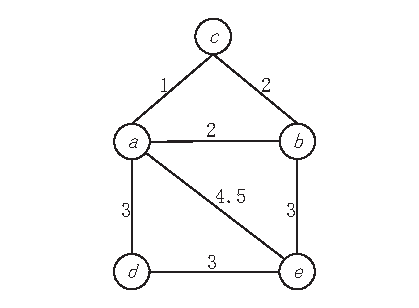
\includegraphics[width=1.3in]{lfaexample}
\caption{An example for explaining LFA}
\label{lfaexample}
\end{figure}


%LFC can protect against a single link failure, NPC can protect against a
%single node failure, while DC is applicable to more complex failure scenarios.
%We will now dive into the details of LFA.

\textbf{LFC:}
$x$ can be chosen when $C_x(d)\!<\!C_x(c)\!+\!C_{c}(d)$,
which means when packets are routed from $x$ to $d$, they will not be routed back to $c$,
since $C_{x}(c)+C_{c}(d)$ is the lowest cost of any path from $x$ to $d$ that passes $c$.
So the protection route will bypass $c$, thus bypass link $(c,b)$ too.

\textbf{NPC:}
$x$ can be chosen when $C_x(d)<C_x(b)+C_b(d)$,
which means the protection route will bypass $b$, thus also bypass link $(c,b)$.

\textbf{DC:}
$x$ can be chosen when $C_x(d)<C_c(d)$,
which means the protection route will bypass $c$ (and link $(c,b)$),
and the remaining cost to the destination strictly decreases.

From the explanation above, we can see all of the three criteria can bypass a link failure,
while \textbf{NPC} can also bypass a node failure.
In addition, \textbf{DC} has a nice property that even when used simultaneously by multiple nodes,
there will be no loop due to the decreasing cost to the destination,
while \textbf{LFC} and \textbf{NPC} can only be used by node $c$ locally.
This property makes \textbf{DC} useful in building multipath routing algorithms \cite{TBFH, dmpa, Yang_Source:2006}.


As in the concrete example of Fig. \ref{lfaexample}, let $c$ be the computing node.
For all packets destined to $d$,
$c$ selects node $b$ as its default next hop.
Since $C_a(d)=5, C_{a}(c)=2$, and $C_{c}(d)=4$, node $a$ satisfies \textbf{LFC}, i.e., $C_a(d)<C_a(c)+C_c(d)$,
and can be used as an alternate next hop if the link $(c,b)$ fails.
However, node $a$ does not satisfy \textbf{NPC} since $C_a(d)=C_a(b)+C_b(d)$,
so if the failed component is node $b$, $a$ cannot be used as an alternate.
Similarly, since $C_a(d)>C_c(d)$, $a$ cannot be used in \textbf{DC} based multipath routing schemes.

Now consider another destination $e$, and the default next hop on $c$ for destination $e$ will now be $a$.
Since $C_b(e)<C_b(c)+C_c(e)$, $C_b(e)<C_b(a)+C_a(e)$, and $C_{b}(e)<C_{c}(e)$,
$b$ is a valid next hop for destination $e$ according to anyone of \textbf{LFC}, \textbf{NPC}, and \textbf{DC},
so it can be used for local route protection from link failure and node failure,
and for \textbf{DC} based  multipath routing.


%Since the performance of routing and forwarding is critical to the Internet, routing protection algorithm has to be highly efficient to avoid becoming a bottleneck. However, the existing approaches often focus on finding more, or  disjoint paths, rather than reducing the computation or the communication overhead, which is the focus of this paper.

\iffalse In \cite{dmpa}, we propose a shortest path tree based multipath routing
algorithm called DMPA. DMPA guarantees loop-freeness of
the induced routing path by implicitly maintaining a partial
order of the routers underpinning it The time complexity of
DMPA does not depend on the degree of the calculating router.
However, the protection ration of DMPA is still lower than
the DC.
Unlike the above works, however, our main concerns are computational efficiency and network availability, as these are critical for the routing protection algorithm. Based on the existing work on this research area, we for the first time propose two routing protection algorithms (IAC and IAC) whose complexity is less than that of Dijkstra��s algorithm and also have a high network availability.

Unlike the above works, however, our main concerns
are computational efficiency and protection ratio, as these are
critical for the Algorithm. Based on the existing work on this
research area, we for the first time propose an algorithm whose
complexity is less than that of Dijkstras algorithm and without
degrading the protection ratio.
\fi

%Unlike the above works, however, our main concerns are computational efficiency and network availability, as these are critical for the routing protection algorithm. Based on the existing work on this research area, we for the first time propose a routing protection algorithm whose complexity is less than that of Dijkstra��s algorithm and also has a high network availability.
